\documentclass[3p, sort&compress]{elsarticle}
\usepackage{titlesec}
\usepackage{typed-checklist}
\titleformat{\paragraph}[runin]{%
    \normalsize\itshape\bfseries}{\theparagraph}{1em}{}
\titlespacing*{\paragraph}{0pt}{%
    3.25ex plus 1ex minus .2ex}{\the\fontdimen2\font}
\usepackage[utf8]{inputenc}
\usepackage{amsmath}
\usepackage{amssymb}{}
\usepackage{amsthm}
\usepackage{enumitem}
\usepackage{lineno, hyperref}
\usepackage{listings}
\usepackage{booktabs}
\usepackage{siunitx}
\usepackage{graphicx}
\usepackage[nameinlink,noabbrev]{cleveref}
\usepackage[draft]{changes}
\usepackage[section]{placeins}
\usepackage[]{algorithm,algcompatible,lipsum}
\usepackage[]{algpseudocode}
\usepackage{scrextend}
\usepackage{changes}
%
\modulolinenumbers[1]
\definechangesauthor[color=orange]{SDIV}
\linenumbers
\newdefinition{hypotheses}{Hypothesis}
\newdefinition{assumptions}{Assumptions}
\newdefinition{rmk}{Remark}
\graphicspath{{./Figures/}{./figs/}}
\begin{document}
    %!TEX root = main.tex
\begin{frontmatter}
    \title{
        Optimal piecewise constant vaccination and lockdown
        policies for COVID-19
    }
    %%%%%%%%%%%%%%%%%%%%%%%%%%%%%%%%%%%%%%%%%%%%%%%%%%%%%%%%%%%%
    \author[add:unison]%
    {Gabriel A. Salcedo-Varela
    % orcid:0000-0002-0147-5089
    }
    \ead{a211203745@unison.mx}
    \address[add:unison]{
        Departamento de Matem\'aticas, Universidad de Sonora,
        Blvd. Luis Encinas y Rosales S/N,
        Hermosillo, Sonora, M\'exico, C.P. 83000.
    }
    %%%%%%%%%%%%%%%%%%%%%%%%%%%%%%%%%%%%%%%%%%%%%%%%%%%%%%%%%%%%%%%%
    \author[add:UADY]%
    {F. Pe\~nu\~nuri}
    \ead{francisco.pa@correo.uady.mx}
    \address[add:UADY]{Facultad de Ingenier\'ia, Universidad
    Aut\'onoma de Yucat\'an, A.P. 150, Cordemex, M\'erida, Yucat\'an,
    M\'exico.}
    %%%%%%%%%%%%%%%%%%%%%%%%%%%%%%%%%%%%%%%%%%%%%%%%%%%%%%%%%%%%%%%%
    \author[add:conacyt_unison]{D. Gonz\'alez-S\'anchez}
    \ead{dgonzalezsa@conacyt.mx}
        \address[add:conacyt_unison]{
        CONACYT-Universidad de Sonora,
        Departamento de Matem\'aticas,
        Blvd. Luis Encinas y Rosales S/N,
        Hermosillo, Sonora, M\'exico, C.P. 83000.
    }
    %%%%%%%%%%%%%%%%%%%%%%%%%%%%%%%%%%%%%%%%%%%%%%%%%%%%%%%%%%%%%%%%
    \author[add:conacyt_unison]{%
        Sa\'ul D\'iaz-Infante%
        \corref{corresponding_author}%
    }%
    \ead{saul.diazinfante@unison.mx}
    %%%%%%%%%%%%%%%%%%%%%%%%%%%%%%%%%%%%%%%%%%%%%%%%%%%%%%%%%%%%%%%
    \cortext[corresponding_author]{Corresponding author}
    \begin{keyword}
        COVID-19, Optimal Control, Lockdown, vaccine,
        Vaccination, WHO-SAGE, DALYs.
    \end{keyword}
    %!TEX root = main.tex
\begin{abstract}
    We formulate a controlled system of ordinary differential equations, with 
vaccination and lockdown interventions as controls, to simulate the mitigation 
of COVID-19. The performance of the controls is measured through a cost 
functional involving vaccination and lockdown costs as well as the burden of 
COVID19 quantified in DALYs. We calibrate parameters with data from Mexico City 
and Valle de Mexico.  By using differential evolution, we minimize the cost 
functional subject to the controlled system and find optimal policies that are 
constant in time intervals of a given size. The main advantage of these 
policies relies on its practical implementation since the health authority has 
to make only a finite number of different decisions. Our methodology to find 
optimal policies is relatively general, allowing changes in the dynamics, the 
cost functional, or the frequency the policymaker changes actions.
\end{abstract}

    \journal{Applied Mathematics and Computation}
\end{frontmatter}
    \section{Introduction}
        %!TEX root = main.tex
%BACKGROUND

    At the date of writing this manuscript, the USA is running its COVID-19 Vaccination
with Pfizer-BioNTech vaccine. This vaccine development, along with Astra-Zeneca, 
Cansino, Sputnik V, and Novavax, promises to deliver enough doses for Latin America.
In Mexico, particularly, the first stock with around 40 000 shots has arrived past
Christmas. In past October, WHO established a recommended protocol for prioritizing
access to this pharmaceutical hope, giving clear lines about who has to be vaccinated
first and why. However, each developed vaccine implies different issues around its 
application. For example, the Pfizer-BioNTech vaccine requires two doses and particular
logistics requirements that demand special services. In Mexico, despite Pfizer-BioNTech,
has been taking the responsibility to capacitate personnel that manages the Vaccination,
there is an explicit demand for logistics resources that limit the institutions' response. 
On the other hand, nonpharmaceutical interventions (NPIs), like Lockdown, mobility reduction, 
social distancing, and other restrictions, also involve economic costs.  

    Our research in this manuscript explores the effect of two interventions, 
Vaccination and Lockdown, to mitigate the  propagation of COVID-19.
We claim that this combined strategy would improve the mitigation of the current pandemic
and also would protect the economic harsh that implies the implementation of Lock-downs.


    Among the related literature about the two interventions we deal with in this paper, 
we can mention the following. The problem of who is vaccinated first, when the number
of available shots is limited, has been transformed into an optimal allocation problem
of vaccine doses in \cite{Bubar2020,Matrajt2020,Buckner2020}.  
These articles face the critical question:  how much doses allocate to each different
group according to risk and age to minimize the burden of COVID-19. Our study takes
the allocation for granted and modulates vaccination and lockdown-release rates as
a combined strategy. Further, papers modeling NPIs consider the diminish of contact 
rates by reducing mobility or modulating parameters regarding the generation of new
infections by linear controls \cite{Naraigh2020,Ullah2020},
lockdown--quarantine \cite{Mandal2020}, and shield immunity
\cite{Weitz2020}. Also, Libotte et al. report in \cite{Libotte2020} optimal vaccination
strategies for COVID-19.  
 
    Since health services' response will be limited by the vaccine stock
and logistics costs, implementing in parallel NPIs is imminent. We focus on
formulating and studying via simulation a lockdown-vaccination system by 
consider the vaccine recently approved by  Mexico Health Council.
We aim to design a dose application schedule subject to a given vaccine 
stock applied in a given period. For this purpose, we formulate an 
optimal control problem that minimizes the burden of  COVID-19 in DALYs 
\cite{WhoDALY}, the cost generated by   running the vaccination 
campaign, and economic damages due to lockdown.

    One of the main features of our model is that we consider piecewise
constant control policies instead of general measurable control 
policies\textemdash also called permanent controls\textemdash to minimize a cost 
functional. General control policies are difficult to implement since the 
authority has to make different choices every permanently. The optimal policies 
we find are constant in each interval of time and hence these policies are 
easier to implement. To the best of our knowledge, our manuscript is the first 
optimal control model with both lockdown and vaccination strategies. 


In \Cref{sec:Covid19_spread}, we formulate the
basic spread model for COVID19 and calibrate its parameters. Then,
\Cref{sec:vaccination_model} establishes the lockdown--vaccination model and
discusses the regarding reproductive number in
\Cref{sec:reproductive_number}. 
In \Cref{sec:optimal_controlled} we describe the optimal control problem 
which consists in minimizing a cost functional subject to controlled 
lockdown--vaccination system. The optimal policies we find, by solving 
numerically the optimal control problem, are presented in 
\Cref{sec:numerical_experiments}. We conclude with some final comments in 
\Cref{sec:discussion}.





\begin{center}
    \textcolor{blue}{\bf Alternative intro}
\end{center}

1. Definition of the topic plus background.
mitigate the pandemic with NPIs 

there is a vaccine scarcity, handling costs, not sure immunity   

a full lockdown yields a negative economic impact, evidence about the GDP

how to balance both policies

implications in the cost functional

2. Accepted state of the art plus problem to be resolved.


there are many works of covid-19 spread, 
allocation of doses by priority group 
there also works on optimization including vaccination or lockdown separately but our paper focuses on both policies
PROBLEM TO RESOLVE:
    Previous work olnly  consider separately vaccination or lockdown policies, but not syncronized or balanced with economical implications.


3. Authors’ objectives.

    Our research in this manuscript explores the effect of two interventions, 
%Vaccination and Lockdown, to mitigate the  propagation of COVID-19.
claims that  combined and synchronized strategy of Lockdown and vaccinating
would improve the mitigation of the current pandemic
and also would protect the economic harsh that implies the implementation of Lock-downs.

    Since health services' response will be limited by the vaccine stock
and logistics costs, implementing in parallel NPIs is imminent. We focus on
formulating and studying via simulation a lockdown-vaccination system by 
consider the vaccine recently approved by  Mexico Health Council.
We aim to design a dose application schedule subject to a given vaccine 
stock applied in a given period. For this purpose, we formulate an 
optimal control problem that minimizes the burden of  COVID-19 in DALYs 
\cite{WhoDALY}, the cost generated by   running the vaccination 
campaign, and economic damages due to lockdown.

4. Introduction to the literature. 
    Corner stone articles [SAUL] (one paragraph)
5. Survey of pertinent literature (optimal vaccination)

    Among the related literature about the two interventions we deal with in this paper, 
we can mention the following. The problem of who is vaccinated first, when the number
of available shots is limited, has been transformed into an optimal allocation problem
of vaccine doses in \cite{Bubar2020,Matrajt2020,Buckner2020}.  
These articles face the critical question:  how much doses allocate to each different
group according to risk and age to minimize the burden of COVID-19. Our study takes
the allocation for granted and modulates vaccination and lockdown-release rates as
a combined strategy. Further, papers modeling NPIs consider the diminish of contact 
rates by reducing mobility or modulating parameters regarding the generation of new
infections by linear controls \cite{Naraigh2020,Ullah2020},
lockdown--quarantine \cite{Mandal2020}, and shield immunity
\cite{Weitz2020}. Also, Libotte et al. report in \cite{Libotte2020} optimal vaccination
strategies for COVID-19.  


%6 authors’ contribution 
%7 aim of the present work 
    We aim optimal and synchronized lockdown-vaccination 
policies that indicates when and how many people 
have to be vaccinated or isolated in order to minimize 
deaths, infected prevalence and economical impact.

% 8 main results / conclusions

   One of the main features of our model is that we consider piecewise
constant control policies instead of general measurable control 
policies\textemdash also called permanent controls\textemdash to minimize a cost 
functional. General control policies are difficult to implement since the 
authority has to make different choices every permanently. The optimal policies 
we find are constant in each interval of time and hence these policies are 
easier to implement. To the best of our knowledge, our manuscript is the first 
optimal control model with both lockdown and vaccination strategies. 


%9 future implications


%10 outline of structure 

In \Cref{sec:Covid19_spread}, we formulate the
basic spread model for COVID19 and calibrate its parameters. Then,
\Cref{sec:vaccination_model} establishes the lockdown--vaccination model and
discusses the regarding reproductive number in
\Cref{sec:reproductive_number}. 
In \Cref{sec:optimal_controlled} we describe the optimal control problem 
which consists in minimizing a cost functional subject to controlled 
lockdown--vaccination system. The optimal policies we find, by solving 
numerically the optimal control problem, are presented in 
\Cref{sec:numerical_experiments}. We conclude with some final comments in 
\Cref{sec:discussion}.


    \section{Covid-19 spread dynamics}
        \label{sec:Covid19_spread}
        %!TEX root = main.tex
    We split a given population of size $N$ in the basic SEIR
structure with segregated classes according to the manifestation
of symptoms. Let $L, S, E, I_S, I_A, H, R, D$ respectively denote the
class of individuals according to their current state, namely
%
\begin{description}[%
    labelwidth=\widthof{\textbf{Infected-Asymptomatic $(I_A)$}},
    leftmargin=\widthof{\textbf{Infected-Asymptomatic $(I_A)$}},
    align=right%
]
    \item[Lockdown $(L)$:]
        All individuals that have low or null mobility and remain under
        isolation. Thus individuals in this class reduce their contagion probability.
    \item[Susceptible $(S)$:]
        Individuals under risk.
    \item[Exposed $(E)$:]
        Population fraction that hosts SARS-CoV-2 but cannot infect.
    \item[Infected-Symptomatic $(I_S)$:]
        Population infected fraction with symptoms and reported as confirmed
        cases.
    \item[Infected-Asymptomatic $(I_A)$:]
        Infected individuals with transitory or null symptoms and unreported.
    \item[Hospitalized $(H)$:]
        Infected population that requires hospitalization or intensive care.
    \item[Recover or removed $(R)$:]
        Population that recovers from infection and develops partial immunity.
    \item[Death $(D)$:]
        Population fraction that died due to COVID-19.
\end{description}
%
To fit data of cumulative reported symptomatic cases, we
postulate the counter state $Y_{I_S}$ and make the following assumptions.
%
%
\begin{assumptions}
    According to above compartment description, we made the following
    hypotheses.
    \begin{enumerate}[label={(A-\arabic*)}]
        \item
            We suppose that at least \SI{30}{\percent} of the population is
            locked down and a fraction of this class eventually moves
            to the susceptible compartment at rate $\delta_L$.
        \item
            Force infection is defined as the probability of acquiring COVID-19
            given the contact with a symptomatic or asymptomatic individual.
            Thus we normalize with respect to alive population population
            $
                N^{\star}
            $.
        \item
            Susceptible individuals become
            exposed\textemdash but not infectious\textemdash
            % exposed individuals
            %host the virus but can not transmit it.
            when they are in contact with asymptomatic or symptomatic
            individuals. Thus $\beta_S$ and $\beta_A$ denote the
            probabilities of being infectious given the contact with a symptomatic or
            asymptomatic infectious individuals, respectively.
        \item
            After a period of latency  $1/\kappa = \SI{5.1}{days}$, an
            exposed individual becomes infected. Being $p$ the probability of
            developing symptoms and $(1-p)$ the probability of becoming infectious
            but asymptomatic. Thus $p\kappa E$ denotes the
            exposed individuals that become infectious and develop symptoms.
        \item
            Asymptomatic individuals do not die or stay in the hospital.
        \item
            A fraction $\mu_{H}$ of symptomatic individuals
            dies due to COVID-19 without hospitalization.
        %\item
    \end{enumerate}
\end{assumptions}

\begin{figure*}[tbh]
    \centering
      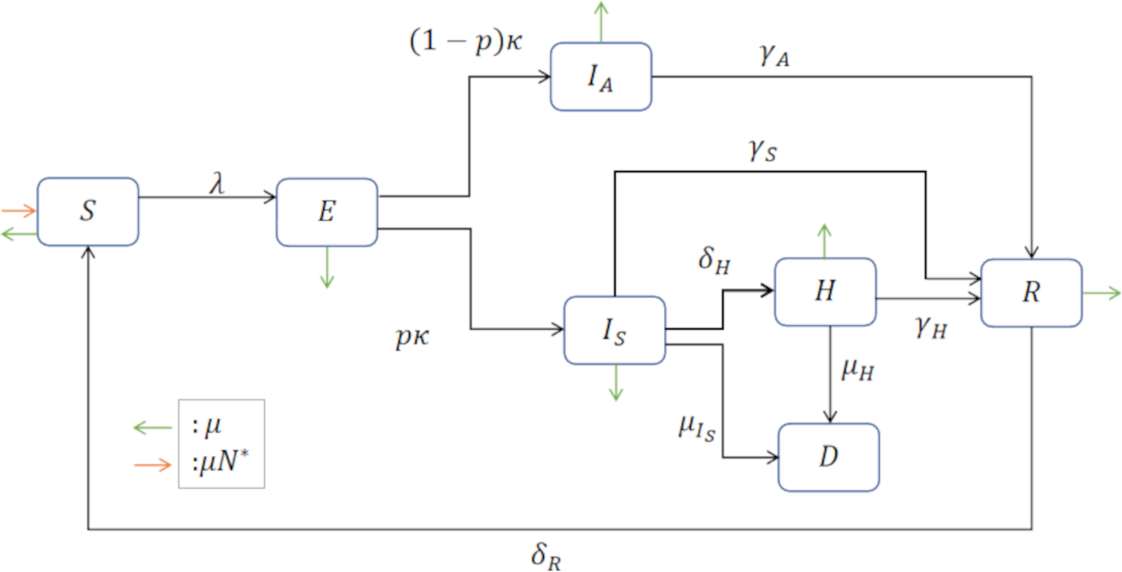
\includegraphics[scale=0.9, keepaspectratio]{Diagram_no_Vaccination.pdf}
    \caption{Compartmental diagram of COVID-19 transmission dynamics. Consider the class: Susceptible $(S)$, exposed $(E)$, symptomatic infected $(I_S)$, asymptomatic 
        infected $(I_A)$, recovered $(R)$, death $(D)$ and vaccinated $(V)$ 
        individuals. It is important to mention that $I_{S}$ represents the 
        proportion of symptomatic individuals who will later report 
        to some health medical center.}
    \label{fig:diagramnolockdownandVacc}
\end{figure*}

Thus we formulate the following Ordinary Differential Equation (ODE), see
\Cref{fig:diagramnolockdownandVacc}, to complete the underlying description.
\begin{equation}
	\label{eqn:base_dynamics}
    \begin{aligned}
        S' & =
            \mu N^\star + \delta_R R - (\lambda + \mu)
            S,
        \\
        E' & =
            \lambda (\epsilon L + S) - (\kappa + \mu) E,
        \\
        I_S' & =
            p \kappa E -
            (\gamma_S +
                \delta_H +
                \mu_{I_S} +
                \mu) I_S,
        \\
        I_A' &=
            (1 - p) \kappa E - (\gamma_A + \mu) I_A,
        \\
        H' &=
            \delta_H I_S - (\gamma_H + \mu_H + \mu) H,
        \\
        R' & =
            \gamma_S I_S + \gamma_A I_A + \gamma_H H - (\delta_R + \mu) R,
        \\
        D' &=
            \mu_{I_S} I_S + \mu_H H,
        \\
        \frac{dY_{I_S}}{dt} &  = p \kappa E,
        \\
        \lambda &:=
            \frac{\beta_A I_A + \beta_S I_S}{N^{\star}},
        \\
        N^{\star}(t) &=
            L + S + E +
            I_S + I_A +
            H + R .
    \end{aligned}
\end{equation}
%
\begin{figure}
    \begin{center}
        \includegraphics[scale=0.25,
        keepaspectratio]{no_contraled_dynamics}
    \end{center}
    \caption{
        Spreed dynamics of COVID-19 according to model in
        \Cref{eqn:base_dynamics}.
    }
    \label{fig:base_dynamics}
\end{figure}

    We display in \Cref{fig:base_dynamics} a typical evolution of this COVID-19 spreed dynamics.
\Cref{tbl:dynamics_base_parameters} encloses notation and reference values.
%
\begin{table*}[h!]
	\centering
	\begin{tabular}{>{\centering}%
        p{0.2\textwidth}%
        p{0.4\textwidth}
    }
    \toprule
		\textbf{Parameter} & \textbf{Description}
  	\\
  	\midrule
		$\mu$ &
			Death rate
		\\
        $\beta_S$ &
        	Infection rate between susceptible and symptomatic infected
		\\
        $\beta_A$ &
        	Infection rate between susceptible and asymptomatic infected
		\\
        $\lambda_V$ &
        	Vaccination rate
		\\
        $\delta_{V}^{-1}$ &
        Vaccine-induced immunity
		\\
        $\varepsilon$ &
        	Vaccine efficacy
		\\
        $\kappa^{-1}$ &
        	Average incubation time
        \\
		$p$ &
			New asymptomatic generation proportion
		\\
	    $\theta$ &
        	Proportion of suceptible individuals under lockdown
        \\
        $\gamma_{S}^{-1}$ &
        	Average time of symptomatic recovery
        \\
		$\gamma_{A}^{-1}$ &
			Recovery average time of asymptomatic individuals
		\\
		$\gamma_{H}^{-1}$ &
			Recovery average time by hospitalization
		\\
        $\delta_{R}^{-1}$ &
        	Natural immunity
  		\\
  		$\delta_{H}$ &
        	Infected symptomatic hospitalization rate
  		\\
  	\bottomrule
	\end{tabular}
		\caption{
			Parameters definition of model in
			\Cref{eqn:base_dynamics}.}
    \label{tbl:dynamics_base_parameters}
\end{table*}
%
\begin{figure*}[htb]
    \centering
    \includegraphics[scale=0.8, keepaspectratio]{Figures/cdmx_input_data}
    \caption{%
        Cumulative new symptomatic and confirmed COVID19 reported cases from
        Ciudad de Mexico and Valle de Mexico
        \cite{cdmxDATA} between March, 10, to March 30 of
        2020.
        \href{https://plotly.com/~AdrianSalcedo/48/}{%
		https://plotly.com/~AdrianSalcedo/48/}
	}
    \label{fig:data_CDMX}
\end{figure*}
%

        \subsection{Parameter calibration}
            \input{parameters_callibration}
    \section{Imperfect-preventive COVID-19 vaccination}
        \label{sec:vaccination_model}
        %!TEX root = main.tex
%
\begin{assumptions}
     According to COVID-19 dynamics \Cref{eqn:base_dynamics}, we
     made the following modeling hypotheses about the regarding vaccine.
     \begin{enumerate}[label={\textbf{(VH-\arabic*)}}]
        \item
            Vaccine is preventive and only reduce susceptibility.
            
        \item
            The vaccination camping omits testing to detect seroprevalence.
            Thus Exposed, Infected Asymptomatic and Recovered Asymptomatic
            individuals are undetected but would obtain a vaccine dose
            \textemdash which in this model represents a waste of resources
        \item
            Individuals under lockdown are also vaccinated
        \item
            The vaccine is leaky and with efficacy $\epsilon \in[0.7, .975]$
        \item   
            Vaccine induced immunity last \SI{2}{years}
        \item   
            Natural immunity last a period of \SI{180}{days} 
     \end{enumerate}
\end{assumptions}
\begin{figure*}[tbh]
    \centering
      \includegraphics[scale=0.7, keepaspectratio]{Diagram_Vaccination.pdf}
    \caption{Compartmental diagram of COVID-19 transmission dynamics which 
        including vaccination dynamics. Here, we consider the Lockdown class $(L)$.}
    \label{fig:diagram_vaccination}
\end{figure*}

\begin{equation}
    \label{eqn:vacination_dynamics}
    \begin{aligned}
        L' =&  \theta \mu N^{\star}
                -(\epsilon \lambda + \delta_L + \lambda_V +\mu) L
        \\
        S' =&
            (1 - \theta) \mu N^\star
            + \delta_L L
            + \delta_V V
            + \delta_R R
            \\
            &-
            \left(
                \lambda + \lambda_V + \mu
            \right) S
        \\
        E' =&
                \lambda (\epsilon L + (1-\varepsilon) V + S)
                - (\kappa + \mu) E
        \\
        I_S' =&
            p \kappa E
            -
            (
                \delta_H +
                \gamma_S +
                \mu_{I_S} +
                \mu
            ) I_S
        \\
        I_A' = &
                (1 - p) \kappa E - (\gamma_A + \mu) I_A
        \\
        H' = &
            \delta_H I_S - (\gamma_H + \mu_H + \mu) H
        \\
        R' = &
            \gamma_S I_S +
            \gamma_A I_A +
            \gamma_H H
                - (\delta_R + \mu) R
        \\
        D'  = &
                \mu_{I_S} I_S + \mu_H H
        \\
        V' = &
            \lambda_V  (S + L)
            - \left[
                (1 - \varepsilon) \lambda
                + \delta_V
                + \mu
            \right ] V
        \\
        \\
            \frac{dX_{vac}}{dt}
                &=
                (u_V(t) + \lambda_V)
                \left[
                    L + S + E + I_A + R
                \right]
        \\
            \frac{d Y_{I_S}}{dt}
                & = p \kappa E
        \\
            \lambda &:=
                \frac{\beta_A I_A + \beta_S I_S}{N^{\star}}
        \\
        \\
            L(0) &= L_0,
            \ S(0) = S_0,
            \ E(0) = E_0,
        \\
            I_S(0) &= I_{S_{0}},
            I_A(0) = I_{A_{0}},
            H(0) = H_0,
        \\
            R(0) &= R_0, \ D(0) = D_0,
      \\
            V(0) &= 0, \ X_{vac}(0) = 0, \quad
      \\
            X_{vac}(T) &= x_{coverage},
      \\
            N^{\star}(t) &=
                L + S +E + I_S + I_A +
                H + R + V .
        \end{aligned}
\end{equation}

    \section{Lockdown-Vaccination reproductive number}
        \label{sec:reproductive_number}
        %\paragraph{$R_0$ definition}
%
The basic reproductive number, which is generally denoted by $ R_0 $,
is a threshold quantity  we can  
 control with particular strategies. The epidemiological interpretation of 
$ R_0 $ is the average number of secondary cases produced by an infected
individual introduced into a population of susceptible individuals.
Using van den Driessche's \cite{VandenDriessche2017a} definition of reproductive number
we obtain
\begin{equation*}
    \label{eqn:reproductive_number}
    \begin{aligned}
        R_0 :=
        &
        \frac{\kappa}{(\kappa + \mu)(\delta_L + \mu)}
        \left(
            \mu R_1 + \delta_L
        \right)
        \left[
            \frac{p\beta_S}{R_2}
            +\frac{(1 - p) \beta_A}{\gamma_A+\mu}
        \right],
    \\
    \text{where} &
    \\
        R_1 &= 1 - \theta(1 - \epsilon),
    \\
        R_2 &= \mu + \delta_H + \gamma_S + \mu_{I_{S}}.
    \end{aligned}
\end{equation*}
%
The factor $\frac{p\beta_S}{R_2}$ measures the proportion of new infections
generated by a symptomatic infectious individual in the time that it lasts
infected. In a similar way, the factor $\frac{(1 - p) \beta_A}{\gamma_A+\mu}$
measures the new infections generated by an asymptomatic infectious individual
in the time that it lasts infected. The factor 
$\frac{\mu R_1 + \delta_L}{\delta_L + \mu}$ measures the number
of individuals in lockdown that leave the lockdown, which can be infected.
And finally, the factor $\frac{\kappa}{\kappa + \mu}$ measures
the time of the disease's incubation.
%
If we consider that there is no lockdown, then $ R_0 $ is reduced to
\begin{equation*}
    \label{eqn:reproductive_number_tilde}
    \begin{aligned}
        \tilde{R}_0 :=
        &
        \frac{\kappa}{(\kappa + \mu)}
        \left[
            \frac{p\beta_S}{R_2}
            +\frac{(1 - p) \beta_A}{\gamma_A+\mu}
        \right].
    \end{aligned}
\end{equation*}
%
Note that we have the relation $ R_0 \leq \tilde{R}_0 $. These indicate that there is greater transmission of the disease if there is no lockdown.

%\paragraph{No  vaccine reproductive number}
%\paragraph{Vaccine reproductive number}
%\paragraph{Efficacy, coverage, and vaccination rate}

%\comment[id=SDIV]{%   Here countor plots figure as function of efficacy and    vaccination rate% }
%
%\added[id=SDIV]{Here Gabriel's R not calculations.}
%
Considering Assumptions 2, we can establish a vaccine reproductive number,
in which individuals who have already been vaccinated
can become infected individuals by being in contact with the
symptomatic infected. Using van den Driessche’s \cite{VandenDriessche2017a}
definition of reproductive number and \cite{Alexander2004}, we obtain

\begin{equation*}
 R_{0}^V := \left[ 1-\frac{\varepsilon \lambda_V}
 {\mu+\lambda_V+\delta_V}
 -\frac{\theta\mu(1-\epsilon)}{\mu+\delta_L+\lambda_V}\right]
 (\mu R_1+\delta_L)R_0.
\end{equation*}
%
The threshold quantity $R_0^V$ is the reproductive number of infection
which can be interpreted as the number of infected people produced
by one infected individual introduced into the population in the
presence of vaccination.

%\comment{edit plot range to display level RV=1}
\begin{figure*}[tbh]
    \centering
      \includegraphics[scale=0.6, keepaspectratio]{Figures/Rv_contour}
    \caption{
    Contour plot  of $R_0^V$ as a function of vaccine efficacy $( \varepsilon) $ and
    vaccination rate $(\lambda_V)$ and vaccine-induced immunity average time of half year.
    Orange line represents the value of $\lambda_{Vbase}=\num{0.000611}$, corresponding to a
    coverage $x_{coverage} = \num{0.2}$ and a horizon time $T=\num{365}$ days. 
    Intersection of black line and blue line show a scenario in which it is
        possible to have the $R_0^V=0.65$, considering a vaccine efficacy of 
        \num{0.8} and a vaccination rate 
        of \num{0.7}.}
    \label{fig:rvcontour1}
\end{figure*}

\Cref{fig:rvcontour1} shows $R_0^V$ as a function of vaccine efficacy and vaccination rate. 
The blue line, $ \varepsilon = 0.8 $, tells us what value of $ \lambda_V $ we take  to
have the level curve where $ R_0^V<1 $.

\begin{figure*}[tbh]
    \centering
      \includegraphics[scale=0.7, keepaspectratio]{Figures/NoLockdown_vacc}
    \caption{
        Vaccine efficacy versus vaccination rate feasibility.
        In the purple shaded region $R_0^V<1 $ and in the white region $ R_0^V >1 $. 
        Note that, for this scenario, we consider no lockdown individuals.
    \href{https://plotly.com/~AdrianSalcedo/85/}{%
		https://plotly.com/~AdrianSalcedo/85/}
    }
    \label{fig:Nolockdown}
\end{figure*}

\Cref{fig:Nolockdown} shows the region of vaccine efficacy and vaccination rate, 
for which $R_0^V <1$. In this scenario, there is no lockdown effect. Note that when  vaccine
efficacy is less than 0.2, there is no vaccination rate for which $R_0^V <1$.
In the absence of lockdown individuals, there is a region not feasible for vaccine efficacy
and vaccination rate.

\begin{figure*}[tbh]
    \centering
      \includegraphics[scale=0.7, keepaspectratio]{Lockdown-Vaccination.pdf}
    \caption{
        Vaccine efficacy versus vaccination rate feasibility.
        In the purple shaded region $R_0^V<1 $ and in the white region $ R_0^V >1 $. 
        Note that, for this scenario, we consider lockdown individuals.
        \href{https://plotly.com/~AdrianSalcedo/76/}{%
		https://plotly.com/~AdrianSalcedo/76/}
    }
    \label{fig:Lockdown}
\end{figure*}

\Cref{fig:Lockdown} shows the region for which $R_0^V <1$  when there are lockdown individuals.
In this scenario, we observe that there are values for the vaccine efficacy and vaccination
rate where $R_0^V <1$, which are smaller than the ones we choose in \Cref{fig:Nolockdown}.

    \section{Optimal controlled version}
        \label{sec:optimal_controlled}
        %!TEX root = main.tex
Now we model vaccination, treatment, and lockdown as an optimal control problem.
According to dynamics in \Cref{eqn:base_dynamics}, we modulate the vaccination
rate with a time-dependent control signal  $u_V(t)$. We add
compartment $X_{vac}$
to count all the vaccine applications of lockdown susceptible, exposed,
asymptomatic, and
recovered individuals. This process is modeled by
\begin{equation}
\label{eqn:counter}
  X'(t) =
    (\lambda_V + u_V(t))(L + S + E + I_A + R)
\end{equation}
and describes the number of applied vaccines at time $t$.
Consider
$$x(t):= (L, S, E, I_S, I_A, H, R, D, V, X_{vac})^{\top}(t)$$
and  control signal $u_v(\cdot)$. We quantify the cost and reward of a vaccine
strategy policy via the penalization functional
\begin{equation}
    \label{eqn:cost_functional}
    J(u_L, u_V):=
        \int _0 ^ T
        a_S p \kappa E(r) +
        a_H \delta_H I_s(r) +
        a_D
        \left[
            \mu_{I_S} I_S(r) + \mu_H H(r)
        \right] +
        \frac{1}{2}
        \left[
            c_L u_L^2(r) +
            c_V u_v^2(r)
        \right]
        dr.
\end{equation}
In other words, we assume in functional $J$ that pandemic cost is proportional
to the symptomatic hospitalized and death reported cases and that a vaccination
and lockdown policies implies quadratic consumption of resources.

    Further, since we aim to simulate vaccination policies at different coverage
scenarios, we impose the vaccination counter state's final time condition
$X_{vac}(T)$
\begin{equation}
    \begin{aligned}
      x(T) &= (\cdot, \cdot, \cdot, \cdot, \cdot, X_{vac }(T))^{\top}
      \in \Omega
      \\
      X_{vac}(T)
        &= x_{cover age},
      \\
      x_{coverage}
        & \in
        \left \{
          \text{Low(0.2)},\text{Mid(0.5)}, \text{High(0.8)}
        \right \},
    \end{aligned}
\end{equation}
where $\Omega$ is the positive invariant set
\begin{equation*}
    \begin{aligned}
    \Omega := \left\{ \right. 
        (L, S, E, I_S, I_A, H, R, D, V, X_{vac}) ^{\top} \in [0,1]^{10}
        &: 
        L + S + E + I_S + I_A + H+ R + D + V = 1, 
        \\
        &
        \left.
        \forall t \in [0, T]
    \right\}.
    \end{aligned}
\end{equation*}
    Thus, given the time horizon $T$, we impose that the last fraction of
vaccinated populations corresponds to 20\%, 50\% or 80\%, and
the rest of final states as free. We also impose the path constraint
\begin{equation}
    \label{eqn:path_constrain}
    \Phi(x,t):= H(t) \leq B,
    \qquad \forall t \in [0, T],
\end{equation}
to ensure that healthcare services will not be overloaded. Here $\kappa$
denotes hospitalization rate, and $B$ is the load capacity of a
health system.

\begin{figure*}[tbh]
    \centering
      \includegraphics[scale=0.7, keepaspectratio]{Diagram_Vaccination_control.pdf}
    \caption{ Compartmental diagram of COVID-19 transmission dynamics that includes
    optimal vaccination dynamics, penalization and a path constraint}
    \label{fig:DiagramControl}
\end{figure*}

    Given a fixed time horizon and vaccine efficiency,
we estimate the constant vaccination rate as the solution of
\begin{equation}
    x_{coverage} = 1 - \exp(-\lambda_V T).
\end{equation}
    That is, $\lambda_V$ denotes the constant rate
to cover  a fraction $x_{coverage}$ in time horizon $T$.
Thus, according to this vaccination rate, we postulate a policy $u_v$ that
modulates vaccination rate according to $\lambda_V$ as a baseline. That is,
optimal vaccination amplifies or attenuates the estimated baseline
$\lambda_V$ in a interval $[\lambda_V ^ {\min}, \lambda_V ^ {\max}]$
to optimize functional $J(\cdot)$\textemdash minimizing
symptomatic, death reported cases and optimizing resources.

    Our objective is minimize the cost functional
\eqref{eqn:cost_functional}\textemdash over an appropriated functional
space\textemdash subject to the dynamics in
\cref{eqn:base_dynamics,eqn:counter}, boundary conditions, and the path
constraint in \eqref{eqn:path_constrain}.
That is, we look for vaccination policies $u_V(\cdot)$, which
solve the following optimal control problem (OCP)
\begin{equation}
    \label{eqn:lockdown_vaccination_ocp}
    \begin{aligned}
        \min_{\mathbf{u} \in \mathcal{U}}
            J(u_L, u_V) := &
                \int_0 ^  T
                    a_S p \kappa E(r) +
                    a_H \delta_H I_s(r) +
                    a_D
                    \left[
                        \mu_{I_S} I_S(r) + \mu_H H(r)
                    \right]
                dr +
        \\
                &
                \int_0^T
                    \frac{1}{2}
                    \left[
                        c_L u_L^2(r) +
                        c_V u_v^2(r)
                    \right]
                    dr.
        \\
            \text{s. t.} &
        \\
            L' & =  \theta \mu N^{\star}
                -\epsilon \lambda L - (u_L(t) + \delta_L) L - \mu L
        \\
            S' & =
                (1 - \theta) \mu N^\star
                + (u_L(t) + \delta_L) L
                + \delta_V V
                + \delta_R R
        \\
                & \qquad -
                \left[
                \lambda + (\lambda_V + u_V(t)) + \mu
                \right] S
        \\
            E' &=
                \lambda (\epsilon L + (1-\varepsilon) V + S)
                - (\kappa + \mu) E
        \\
            I_S' &=
                p \kappa E
                % + (1 - q) \gamma_M M(t)
                - (\gamma_S +
                    \mu_{I_S} +
                    \delta_H +
                    %u_M(t) +
                    \mu) I_S
        \\
            I_A' &=
                (1 - p) \kappa E - (\gamma_A + \mu) I_A
        \\
            H' &=
                \delta_H I_S - (\gamma_H + \mu_H + \mu) H
        \\
            R'  &=
                \gamma_S I_S +
                \gamma_A I_A +
                \gamma_H H % +
                - (\delta_R + \mu) R
        \\
            D' &=
                \mu_{I_S} I_S + \mu_H H
        \\
            V' &=
                (\lambda_V + u_V(t)) S
                - \left[
                (1 - \varepsilon) \lambda
                + \delta_V
                + \mu
                \right ] V
        \\
        \\
            \frac{dX_{vac}}{dt}
                &=
                (u_V(t) + \lambda_V)
                \left[
                    L + S + E + I_A + R
                \right]
        \\
            \frac{d Y_{I_S}}{dt}
                & = p \kappa E
        \\
            \lambda &:=
                \frac{\beta_A I_A + \beta_S I_S}{N^{\star}}
        \\
        \\
            L(0) &= L_0,
            \ S(0) = S_0,
            \ E(0) = E_0,
            \ I_S(0) = I_{S_{0}},
      \\
            I_A(0) &= I_{A_{0}},
            H(0) = H_0, \
            \ R(0) = R_0, \ D(0) = D_0,
      \\
            V(0) &= 0, \ X_{vac}(0) = 0, \quad
            u_V(.) \in [u_{\min}, u^{\max}],
      \\
            X_{vac}(T) &= x_{coverage},
      \quad
            \kappa I_S(t) \leq B, \qquad
            \forall t \in [0, T],
      \\
            N^{\star}(t) &=
                L + S +E + I_S + I_A +
                H + R + V
        \end{aligned}
\end{equation}

    \section{Numerical Experiments}
        \label{sec:numerical_experiments}
        %!TEX root = main.tex
\subsection{Methodology}
    We simulate a scenario corresponding to a hypothetical but plausible initial conditions and parameters. We integrate model in
\Cref{eqn:lockdown_vaccination_ocp} by classic Runge Kutta scheme and solve the
optimization stage with the so-called Differntial Evolution method.
Differential Evolution (DE) \cite{Storn1997} is an evolutionary
algorithm successfully employed for global optimization
\cite{Bilal2020}. The method is designed to optimize functions
$f:\mathbb{R}^n \to \mathbb{R}$. Nevertheless, DE can be applied to
optimize a functional as stated in \cite{CANTUNetAl}. The method can be
coded following Algorithm \ref{alg:DE1}, where an initial random
population on the search space $\mathcal{V}$ of size $N_p$ is subjected
to mutation, crossover and selection. After this process a new
population is created which, again would be subjected to the
evolutionary process. This process is repeated until some stopping
criteria is fulfilled. Finally the best individual (according to some
objective function $f_{ob}$ to optimize) is extracted. These operations
are conducted by the operators $\mathbf{X}_0$, $\mathbf{M}$,
$\mathbf{C}$, $\mathbf{S}$, $\mathbf{x}_{best}$;  whose explicit form
are coded in \cite{Penunuri2016}.

In the optimization of this study,
the mutation scale factor $F$ and the crossover probability $C_r$ were
taken as 1 and 0.3 respectively, additional $N_p$ has been taken as 4
times the number of parameters (the dimension of the vector used to
describe the two controls\textemdash see \cite{CANTUNetAl}), which in our case was
of 180. As stopping criteria we have used a maximum number of
generations which is taken as \num{5000}.

    We provide in \cite{gitHub_b} a GitHub repository with all regarding R
and Fortran sources for the sake of reproductivity. This repository also
encloses data sources and a Wolfrang Mathematica notebook to reproduce all
reported figures.
%
%
\begin{algorithm}[htb]
  \caption{Differential Evolution Algorithm}
  \label{alg:DE1}
  \begin{algorithmic}
    % \small
    \State $X \leftarrow \mathbf{X}_0(Np,\mathcal{V})$
    \While{(the stopping criterion has not been met)}
    \State $M \leftarrow \mathbf{M}(X,F,\mathcal{V})$
    \State $C \leftarrow \mathbf{C}(X,M,C_r)$
    \State $X \leftarrow \mathbf{S}(X,C,f_{ob})$
    \EndWhile
    \State $\mathbf{x}_{best} \leftarrow \mathbf{Best}(X, f_{ob})$
  \end{algorithmic}
\end{algorithm}

        %Vaccine development
\begin{figure*}
    \centering
    \includegraphics[scale=0.5, keepaspectratio]{figs/InitialCondition}
    \caption[Initial condition]{
        Initial condition scheme. We assume a positive prevalence. 
        For reference, at the date of write this manuscript, prevalence in CDMX 
        is around \SI{16000}{cases}, see
        \href{https://plotly.com/~sauld/36/}{https://plotly.com/~sauld/36/}
        to display an electronic viewer.}
        \label{fig:initialcondition}
\end{figure*}
\subsection{Simulation}
 According to official Governmental communication in December, Mexico treated  
\num{36000000} doses  Pfizer-Biotech, \num{76000000} doses with Aztra Seneca 
\num{18000000} quantities of Cansino-BIO. Other developments 
also are running the third Phase, and with high probability,  in the third
quarter of 2021, some of these developments will incorporate into Mexico's 
vaccine portfolio. Despite official agreements, each vaccine's delivery schedule 
is under uncertainty and-or subject to the approval of COFEPRIS.

The first accepted vaccine\textemdash Pfizer-BioNTech's BNT162b2\textemdash has 
an efficacy above \SI{90}{\percent} and requires two doses to achieve immunity. 
The other mentioned developments have a very similar profile but require different
logistic management and stock allocation.
Thus, we face designing a dose application schedule subject to a given vaccine stock 
applied in a given period. To this end, we solve the optimal control problem 
\eqref{eqn:lockdown_vaccination_ocp}. We understand as solution of this problem
a pair $(x(\cdot), u(\cdot))$ where
\begin{equation}
    \begin{aligned}
        x(t) &= (L(t), S(t), E(t), I_S(t), I_A(t), H(t), R(t), D(t), V(t))^{\top}
        \\
        u(t) &= (u_L(t), u_V(t)) ^ {\top},
    \end{aligned}
\end{equation}
minimizes the burden of COVID-19 in DALYs \cite{WhoDALY} and the quadratic application
cost of the lockdown-vaccination policy formulated in the functional \eqref{eqn:cost_functional}.  

\subsection*{Simulation Scenario}
\paragraph*{Initial Conditions}
    We assume and a hypothetical scenario where the whole population faces a second wave of COVID-19. 
    Thus whole epidemiological classes have positive prevalence. We also assume that Lockdown and Susceptible 
    compartments initially enclose more than \SI{70}{\percent} of the total population, and the initial
    prevalence of symptomatic cases is below critical levels. Further, under our assumptions, the outbreaks'
    second wave implies a growth accordingly with an Effective Reproductive Number (ERN) 
    above one\textemdash Fig 10 displays a qualitative schematic representation.

%\paragraph{Vaccine profile according to Pfizer}
%    At the moment of writing this manuscipt
%\paragraph{Vaccine-Induced and Natural immunity}
%
%\paragraph{Numerical Experiments}
%
%\paragraph{Results}



\begin{figure*}[tbh]
    \centering
    \includegraphics[width=0.7\linewidth]{figs/lockdown_control_signal}
    \caption[Lockdown modulation signal.]{Lockdown modulation signal.
    \href{https://plotly.com/~AdrianSalcedo/56/}
    {https://plotly.com/~AdrianSalcedo/56/}
            to display a electronic viewer.}
    \label{fig:lockdowncontrolsignal}
\end{figure*}

\begin{figure}
    \centering
    \includegraphics[width=0.7\linewidth]{figs/Vaccination_control_signal}
    \caption[Vaccination rate modulation.]{Vaccination rate modulation.
    \href{https://plotly.com/~AdrianSalcedo/58/}
    {https://plotly.com/~AdrianSalcedo/58/}}
    \label{fig:vaccinationcontrolsignal}
\end{figure}

\begin{figure}[tbh]
    \centering
    \includegraphics[scale=0.65, keepaspectratio]{figs/LockdownEffect}
    \caption{Modulation lock down release.
    \href{https://plotly.com/~AdrianSalcedo/60/}
    {https://plotly.com/~AdrianSalcedo/60/}}
    \label{fig:lockdowneffect}
\end{figure}

\begin{figure*}[tbh]
    \centering
    \includegraphics[scale=0.65, keepaspectratio]{figs/VaccinationEffect}
    \caption{Symptomatic Prevalence and Hozpitalization.
        \href{https://plotly.com/~AdrianSalcedo/61/}
        {https://plotly.com/~AdrianSalcedo/61/}}
    \label{fig:vaccinationeffect}
\end{figure*}

    \section{Discussion}
        \label{sec:discussion}
        \paragraph{Statement of principal finding}
        This study illustrated the implications of applying 
    combined strategies of lockdown and vaccination to mitigate
    the curse of COVID-19. Our experiments suggest that a 
    combined and well-balanced policy between the relaxing 
    times of lockdown and vaccine rollout would improve the 
    mitigation of COVID-19 symptomatic prevalence and deaths,
    but with a delicate balance whit the economic impact. 
    We obtained lockdown policies that modulate individuals' 
    release rate synchronized with the symptomatic prevalence 
    and vaccine rollout speed. Our vaccination policies captured
    time windows where it is convenient to modify the vaccine 
    administration according to the symptomatic prevalence and
    economic cost.
\paragraph{Strengths and weakness of the study}
    %TOPIC SENTENCE
    \begin{CheckList}{Goal}
        \Goal{open}{Argument for Strengths}
            \begin{CheckList}{Task}
                \Task{started}{Piecewise optimal policies}
                \Task{started}{Practical}
                \Task{started}{Modulation between
                    relaxation and inclusion of 
                    population in lockdown}
            \end{CheckList}
    \end{CheckList}

    \paragraph[]{STRENGTHS}
	        We got optimal policies that are practical. 
        Whit practical, we mean those capture actions that can be
	    implemented in the real world. Because the policies rely on 
	    piecewise constant values for a given period (here we use 
	    days), we argue that they are more realistic than policies 
	    that consider continuous functions that could implicate
	    continuous changes of a given action. For example, 
	    it is more realistic to administer a fixed number of jabs
	    along with a given date than following a configuration of
	    several doses that would change continuously on the same date.
    
            Besides, we synchronized the trade of between
        lockdown-release, vaccine-rollout but balancing the 
        economic cost.

    \paragraph[]{WEAKNESS}
        \begin{CheckList}{Goal}
            \Goal{open}{Argument for Weakness}
                \begin{CheckList}{Task}
                    \Task{done}{Vaccine Multi-dose.}
                    \Task{started}{Protection only against severe symptoms.}
                    \Task{started}{What expect respect 
                        to the protection against transmission.
                    }
                \end{CheckList}
        \end{CheckList}
  
            One limitation was the assumption of only one vaccine. 
        In almost all countries the vaccination campaigns consider at 
        least two developments. For example, in Mexico the vaccine portfolio 
        (at the day of writing) relies on at least four developments. Moreover, 
        this vaccine portfolio includes developments that differs in the number 
        of required doses. For example, Pfizers require two doses while Cansino 
        Bio only demands one.
        
            Further, we do not face additional vaccine administration 
        requirements as the time between doses or logistics\textemdash 
        each development implies different protocols. Since the approved 
        vaccine's protective efficacy against transmissions of SARS-CoV2 
        remains under study, we do not consider this hypothesis in our
        formulation. We recognize that this parameter would play an 
        important role, which is plausible to consider in future formulations.

    \paragraph{Strengths and weakness in relation to 
        other studies, discussing important differences
        in results
    }
    \todo{citations}
    \paragraph{STRENGTHS}
        \begin{CheckList}{Goal}
            \Goal{open}{Argument for Weakness}
                \begin{CheckList}{Task}
                    \Task{started}{%
                        NPI's optimal Policies with non Vaccination
                        }
                    \Task{started}{%
                         
                        and compare our results.}
                    \Task{started}{What expect respect 
                        to the protection against transmission.
                    }
                    \Task{open}{Optimal Control of Vaccination Rate
                    cite cite{Libotte2020} and compare our results
                    }
                \end{CheckList}
        \end{CheckList}
        
        Works like 
    \cite{Perkins2020,Palmer2020,Djidjou2020,Asamoah2021,Nabi2021} 
    developed NPI's with optimal control for COVID-19. Some 
    contribution of this list  combines two or more strategies to
    mitigate prevalence and deaths due to SARS-CoV-2. For example,
    \cite{Nabi2021} formulates a fractional ODE model with public
    education, treatment, and management of asymptomatic cases.  
    Assamoth in \cite{Asamoah2021} puts 
    special attention to the economic cost related to the combined 
    health protocol of physical distancing, media advocacy,  
    wearing a mask, hand-washing, lockdown, and contact tracing. 
    Similarly, \cite{Djomegni2021,Jiang2020,Ullah2020}
    reports optimal policies but with significant emphasis on
    other aspects related to the spread dynamics of COVID-19.
    However, the mentioned works developed policies based on
    continuous functions and did not optimize or not include 
    vaccination. In our opinion, these kinds of policies would 
    be impractical for decision-makers. 
	    
	    Here we argue that our policies give a precise sequence 
	of actions that are feasible for implementation. Further, we 
	calculated the cost and balanced its implementation 
	synchronized and balanced with the economic implications.

    \paragraph{WEAKNESS: Static optimization }
        \begin{CheckList}{Goal}
            \Goal{open}{Argument for Weakness}
                \begin{CheckList}{Task}
                    \Task{started}{Allocation.
                        Comment about optimal allocation as a 
                        static optimization problem and cite
                        cite {Bubbar, Buckner, Moore2021}.
                    }
                    \Task{open}{%
                        Other Approach cite and discuss 
                        cite{Lazembink2020}%
                    }
                \end{CheckList}
        \end{CheckList}
    
        On the other hand, another limitation of this work 
	was the lack of stratification and risk groups. Because the 
	year of life lost is susceptible to this regard, and the 
	productive sector of an economy is closely related to the 
	workforce, we might prioritize accordingly. However, we see 
	that our result could complement the prioritization policies 
	of relevant works like \cite{Bubar2021,Matrajt2020a}, Buckner2020].
	While optimal vaccine prioritization strategies answer 
	the question: Who to vaccine first, we answer when intensifying 
	vaccine rollout	and lockdown release. Thus our contribution 
	would be complementary.        

    \paragraph{Meaning of the study: possible explanations 
        and implications for clinicians and policymakers}

        New and more contagious variants of SARS-CoV-2 appeared, 
    and the COVID-19 vaccine supply would be scarce, slow, and 
    complicated for countries like Mexico. Thus we expect three 
    synchronized events: another COVID-19 wave, an
    intensification of the vaccine rollout, and other lockdowns. 
    Here we argued that the above strategies also must be 
    synchronized and consider a delicate balance with the 
    economic impact.

    \paragraph{Unanswered questions and future research}
        
        Despite that NPIs have been implemented in most countries 
    to mitigate COVID-19, these strategies cannot develop immunity. 
    Thus, vaccination becomes the primary pharmaceutical measure. 
    However, this vaccine has to be effective and well implemented 
    in global vaccination programs. Each development implies 
    particular issues--like logistics number of doses, 
    secondary effects, and others. For example, Mexico is 
    administrating vaccines from Pfizer-BioNtech, AstraZeneca, 
    CanSino-Bio, the Sputnik V from Russia, and others. 
    Each of these vaccines implies different requirements 
    for its management, provides protection with different 
    efficacies, and differ in its number of doses. We believe
    that this complicated landscape has significant implications
    in the design of health policies.

        Thus, new challenges in distribution, stocks, politics, 
    vaccination efforts, among others, emerge.     
    
    \section*{Data availability}
            \href{https://github.com/%
        SaulDiazInfante/NovelCovid19-OptimalPiecewiseControlModelling.git}{%
        https://github.com/%
        SaulDiazInfante/NovelCovid19-OptimalPiecewiseControlModelling.git}
    \section*{Authors’ contributions}
    \textbf{Gabriel A. Salcedo-Varela}
    Conceptualization,
    Methodology,
    Software,
    Validation,
    Formal analysis,
    Investigation,
    Resources,
    Visualization,
    Project Administration,
    Writing\textendash original draft,
    Writing\textendash review \& editing.

\textbf{F. Pe\'nu\'nuri}
    Methodology,
    Software,
    Validation,
    Formal analysis,
    Investigation,
    Data curation,
    Visualization,
    Supervision,
    Writing\textendash original draft,
    Writing\textendash review \& editing.

\textbf{David Gonz\'alez-S\'anchez:}
    Conceptualization,
    Methodology,
    Formal analysis,
    Writing\textendash original draft,
    Writing\textendash review \& editing.

\textbf{Sa\'ul D\'iaz-Infante:}
    Conceptualization,
    Methodology,
    Formal analysis,
    Writing\textendash original draft,
    Writing\textendash review \& editing.
        Methodology,
    Software,
    Validation,
    Formal analysis,
    Investigation,
    Data curation,
    Visualization,
    Supervision

    \section*{Conflicts of interest}
    The authors have no competing interests.
    
    \appendix
    \section{Existence of optimal policies}
        %!TEX root = main.tex
In this appendix, we show the existence of optimal policies in the class of
{\it piecewise constant policies}. Consider the following cost functional that
we want to minimize
\begin{equation}\label{costFunctional}
  \int_0^T C(X(t),u(t)) dt
\end{equation}
subject to the dynamics
\begin{equation}\label{dynamics}
  \dot{X}(t) = f(X(t),u(t)),  \qquad    0\leq t \leq T,
\end{equation}
and the initial state $X(0)=x_0$. The functions $u:[0,T]\to U$ are called {\it
control polices}, where $U$ is a subset of some Euclidean space.
    %The
    %cost functional \eqref{eqn:cost_functional} and the dynamics
    %\eqref{eqn:vital_dynamics} are particular cases of \eqref{costFunctional}
    %and \eqref{dynamics}, respectively.
%
Let $t_0<t_1<\ldots <t_n$, with
$t_0=0$ and $t_n=T$, be a partition of the interval $[0,T]$.
We consider piecewise constant policies $\tilde{u}$ of the form
\begin{equation}\label{PieceConstCont}
  \tilde{u}(t) = a_j\qquad t_j\leq t < t_{j+1}
\end{equation}
 for $j=0,\ldots,n-1$.
\begin{assumptions}
    We made the following assumptions.
    \begin{enumerate}[label=\textbf{(ASS-\arabic*)}]
        \item
            The function $f$ in the dynamics \eqref{dynamics} is of
            class $C^1$.
        \item
            The cost function $C$ in \eqref{costFunctional} is continuous and
            the set $U$ is compact.
    \end{enumerate}
\end{assumptions}
%

    By Assumption (A-1)\textbf{}, the system
\[
  \dot{X}(t) = f(X(t),a_0), \quad X(0)=x_0, \qquad    0\leq t \leq t_1,
\]
has a unique solution $\tilde{X}_0(t;x_0,a_0)$ which is continuous in
$(x_0,a_0)$; see, for instance \cite{Kong2014}.  Next, put $x_1:=\tilde{X}_0(t_1;x_0,a_0)$ and consider the system
\[
  \dot{X}(t) = f(X(t),a_1), \quad X(t_1)=x_1, \qquad    t_1\leq t \leq t_2,
\]
Again, by Assumption (A-1), the latter system has a unique solution
$\tilde{X}_1(t;x_1,a_1)$ which is
continuous in $(x_1,a_1)$. By following this procedure, we end up having a
recursive solution
\begin{equation*}
  \begin{aligned}
    & \tilde{X}_{n-1}(t;x_{n-1},a_{n-1}),
    \qquad t_{n-1}\leq t \leq T,\\
    & x_{n-1}:=\tilde{X}_{n-2}(t_{n-1};x_{n-2},a_{n-1}),
  \end{aligned}
\end{equation*}
where $\tilde{X}_{n-1}$ is continuous in $(x_{n-1},a_{n-1})$.


For a control $\tilde{u}$ of the form \eqref{PieceConstCont} and the
corresponding solution path $\tilde{X}$, we have
\[
  \int_0^T
    C(\tilde{X}(t),
    \tilde{u}(t)) dt =
      \sum_{j=0}^{n-1}
        \int_{t_j}^{t_{j+1}}
        C(\tilde{X}_j(t),a_j) dt.
\]
Notice that each $\tilde{X}_j$ is a continuous function of $(a_0,\ldots,a_j)$
and $x_0$.

By Assumption (A-2), the mapping
\[
  (a_0,\ldots,a_{n-1})
  \mapsto
  \sum_{j=0}^{n-1}
  \int_{t_j}^{t_{j+1}} C(\tilde{X}_j(t),a_j) dt
\]
is continuous. Since each piecewise constant policy $\tilde{u}$ of the form
\eqref{PieceConstCont} can be identified with the vector $(a_0,\ldots,a_{n-1})$
in the compact set $U\times\cdots\times U$, the functional
\eqref{costFunctional} attains its minimum in the class of piecewise constant
policies.

    The cost functional \eqref{eqn:cost_functional} and the dynamics
\eqref{eqn:base_dynamics} are particular cases of \eqref{costFunctional} and
\eqref{dynamics}, respectively, and satisfy Assumptions (A-1) and (A-2). Then
there exists an optimal vaccination policy of the form \eqref{PieceConstCont}.
        \bibliography{NovelCovid19.bib}
        %\bibliographystyle{plain}
    \bibliographystyle{elsarticle-num}
\end{document}
